\chapter{Versuchen}
\label{chap:Versuchen}

\section{Untersuchungsplattform}
\label{sec:Untersuchungsplattform}
Unsere Untersuchung wurde durchgeführt auf dem Plattform wie unter:

\begin{table}[htbp]
\begin{center}
\begin{tabular}{ l | l }
	Hardwaresystem 	& ODROID-XU3 Lab Environment(mit ARM Cortex-A7\\
					& 1.4Ghz und Cortex-A15 2.0Ghz big.LITTLE\\
					& architecture jeweils 4 kerne)\\ \hline
	Betribssystem 	& Ubuntu 15.10 mit ssh Zugriff und shared\\
					& storage durch NFS server\\ \hline
	Test-Benchmark 	& NAS Parallel Benchmarks\\ \hline
	Tasks 			& LU Dekomposition und Gauß'sche Elimination(LU)\\ 
					& und konjugierender Gradient(CG)\\ \hline
	Task-Maßstab	& siehe Tablett \ref{tab:Task-Massstab}\\ \hline
	Implementationssprache 	& Java\\ \hline
	Implementationsmethode 	& OpenMP und MPI(Message Passing\\
							& Interface)\\ \hline
	Messungsgeräte & ODROID Smart Power Device 
\end{tabular}
\end{center}
\label{tab:Untersuchungsplattform}
\caption{Untersuchungsplattform}
\end{table}

\begin{table}[htbp]
\begin{center}
\begin{tabular}{l|l|l|l}
	&			&Class A 	&Class B\\ \hline
CG 	&Size		&14000		&75000\\
	&Iteration	&15			&75\\ \hline
LU 	&Size		&64x64x64	&102x102x102\\
	&Iteration	&250		&250\\
\end{tabular}
\end{center}
\label{tab:Task-Massstab}
\caption{Task-Maßstab}
\end{table}

\section{Energiebedarf-relevante Aspekte}
\label{sec:Energiebedarf-relevante Aspekte}

\subsection{Energiebedarf und Architektur}
\label{subsec:Energiebedarf und Architektur}

\begin{figure}[ht]
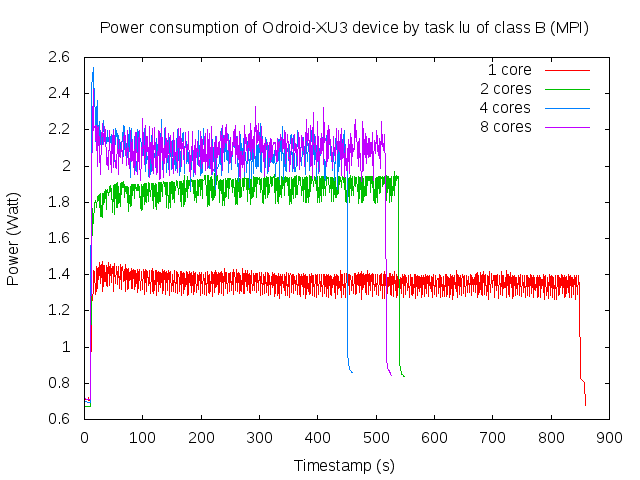
\includegraphics[width=\textwidth]{cores_power}
\caption[Leistung und Kernenutzung]{Leistung und Kernenutzung}
\label{fig:Leistung und Kernenutzung}
\end{figure}

\begin{figure}[ht]
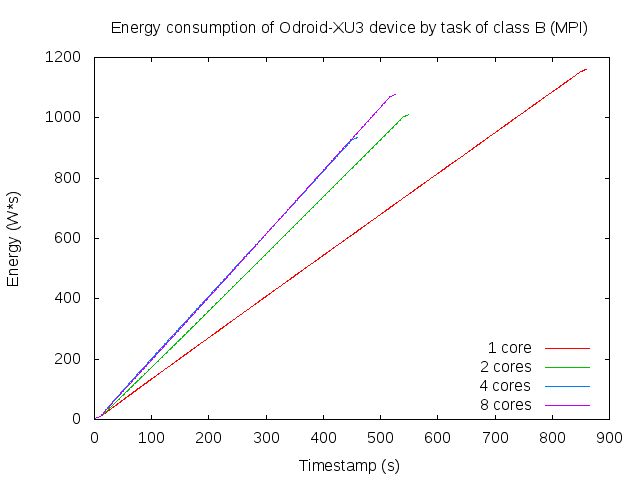
\includegraphics[width=\textwidth]{cores_energy}
\caption[Energiebedarf und Kernenutzung]{Energiebedarf und Kernenutzung}
\label{fig:Energiebedarf und Kernenutzung}
\end{figure}

\begin{figure}[ht]
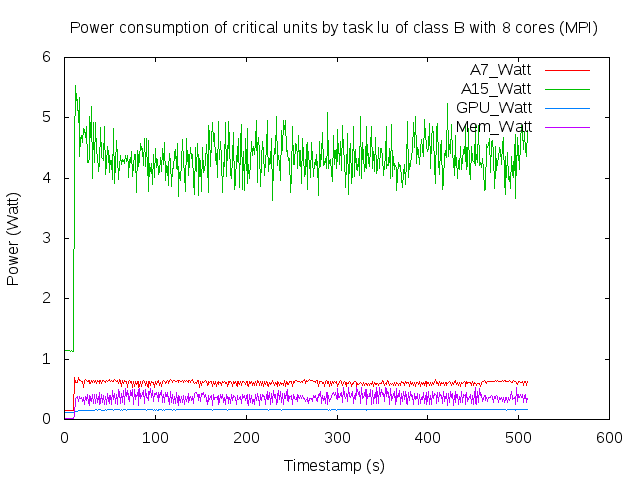
\includegraphics[width=\textwidth]{units_power}
\caption[Leistung kritischer Teilen]{Leistung kritischer Teilen}
\label{fig:Leistung kritischer Teilen}
\end{figure}

Wie gezeigt in Abbildung \ref{fig:Leistung und Kernenutzung} und sein Integral Abbildung \ref{fig:Energiebedarf und Kernenutzung}. Die Rechnung befasst sich um das Task von LU und mit BWenn es nur ein Kern aktiviert ist, ist die Energiebedarf des Computersystems am höchsten und dauert die Rechung am längsten. Deshalb die Konfiguration mit nur ein aktivierende Kern ist auf jeden Fall nicht effizient. 

Aber es ist auch komisch, dass die Zeit- und Energiebedarf des Task von 8 Kerne sind beide höher als die von 4 Kerne. Laut der Dokumentation von ODROID-XU3 kann man feststellen, dass es 4 Kerne von Cortex-A7 und 4 Kerne von Cortex-A15 auf der Tafel sich befindet. Wenn es nur 4 Kerne aktiviert ist, sind die 4 Kerne mit niedrigere ID, d.h. 4 Kerne von Cortex-A7 laufbar. 

Der Grunden dafür kann man mit dem Hilfe Dokumentationen und Versuchergebnisse vermuten. Rechnungsdatenumtauschung innerhalb ein CPU ist immer noch effizienter als die über 2 CPUs. Darum ist die Zeitbedarf mit 4 Kerne nideriger. Beschrieben von Webseite von ARM und in Beachtung von Messungsergebnis in Abbildung \ref{fig:Leistung kritischer Teilen}, ist die Leistung des Cortex-A15 höher als die des Cortex-A7 und für die Energiebedarf vice versa. Deshalb für eine Rechnungsarbeit mit so moderatem Maßtab soll man die energieeffiziente CPUs beforzugen.

\subsection{Energiebedarf und Tasks}
\label{subsec:Energiebedarf und Tasks}

\begin{figure}[ht]
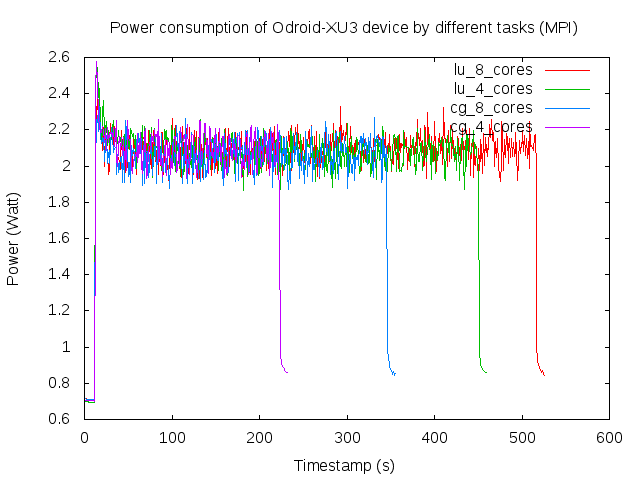
\includegraphics[width=\textwidth]{tasks_power}
\caption[Leistung und Tasks]{Leistung und Tasks}
\label{fig:Leistung und Tasks}
\end{figure}

\begin{figure}[ht]
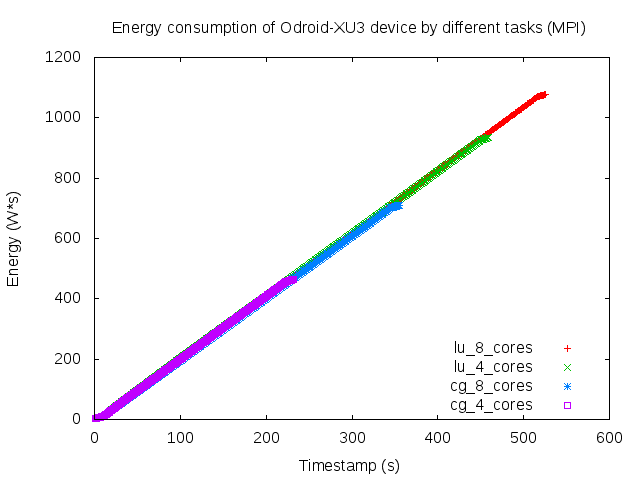
\includegraphics[width=\textwidth]{tasks_energy}
\caption[Energiebedarf und Tasks]{Energiebedarf und Tasks}
\label{fig:Energiebedarf und Tasks}
\end{figure}

Wie hergestellt in Abbildung \ref{fig:Leistung und Tasks} und ihre Integral \ref{fig:Energiebedarf und Tasks}, obwohl sich der gesamte Energiebedarf zwischen verschidenen Tasks und Kernekonfiguraionen sehr viel verändert, gibt es gar keinen Unterschied bezüglich Leistung dazwischen. Dadurch kann man vermuten, dass währen der Versuchen befindet sich jedes CPU nur auf zwei Zustände: aktiviert oder nicht. Es gibt gar keine Zwischenzustand, auf dem ein CPU mit einer unterschiedlicher Leistung ausgeführt werden kann.

\subsection{Energybedarf und Maßstab von Tasks}
\label{subsec:Energybedarf und Massstab von Tasks}

\begin{figure}[ht]
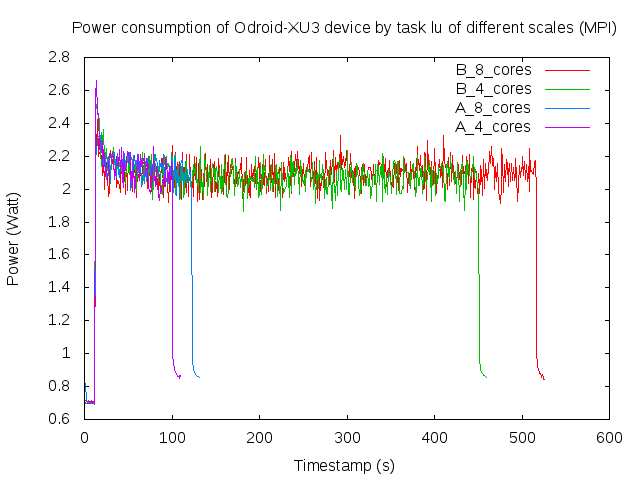
\includegraphics[width=\textwidth]{scales_power}
\caption[Leistung und Maßstab von Tasks]{Leistung und Maßstab von Tasks}
\label{fig:Leistung und Massstab von Tasks}
\end{figure}

\begin{figure}[ht]
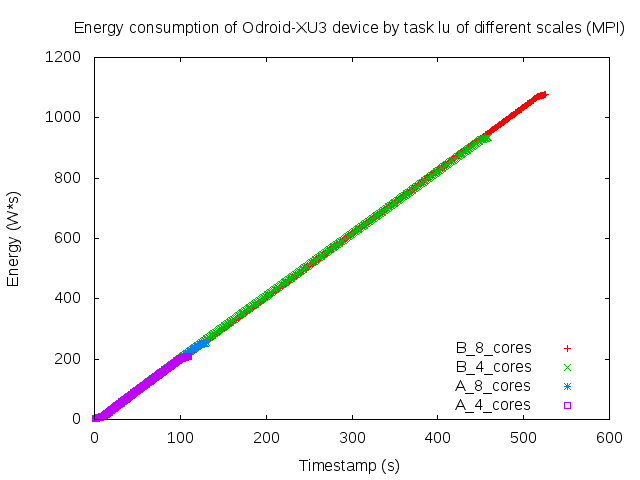
\includegraphics[width=\textwidth]{scales_energy}
\caption[Energiebedarf und Maßstab von Tasks]{Energiebedarf und Maßstab von Tasks}
\label{fig:Energiebedarf und Massstab von Tasks}
\end{figure}

Die Abbildungen \ref{fig:Leistung und Massstab von Tasks} und \ref{fig:Energiebedarf und Massstab von Tasks} zeigen, dass die Maßstäbe der Tasks nichts mit die Leistung des Durchgangs zu tun haben. Nur je größer die Tasks sind, braucht es mehr Zeit die Berechnung zu machen, desto wird mehr Energie insgesamt gebraucht.

\subsection{Energy bedarf und Implementationsmethode}
\label{subsec:Energy bedarf und Implementationsmethode}

\begin{figure}[ht]
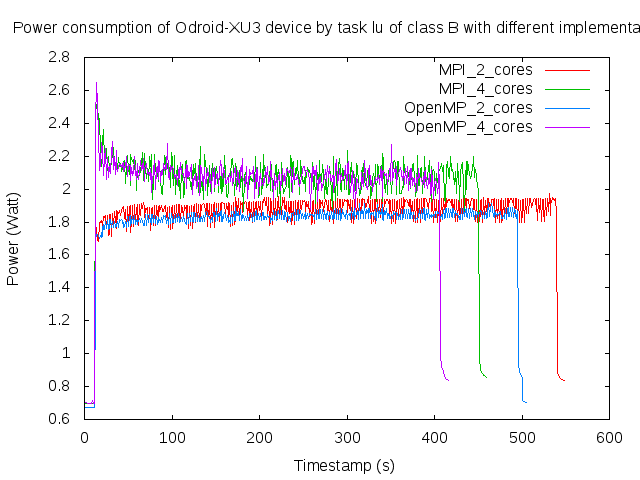
\includegraphics[width=\textwidth]{implementations_power}
\caption[Leistung und Implementationsmethode]{Leistung und Implementationsmethode}
\label{fig:Leistung und Implementationsmethode}
\end{figure}

\begin{figure}[ht]
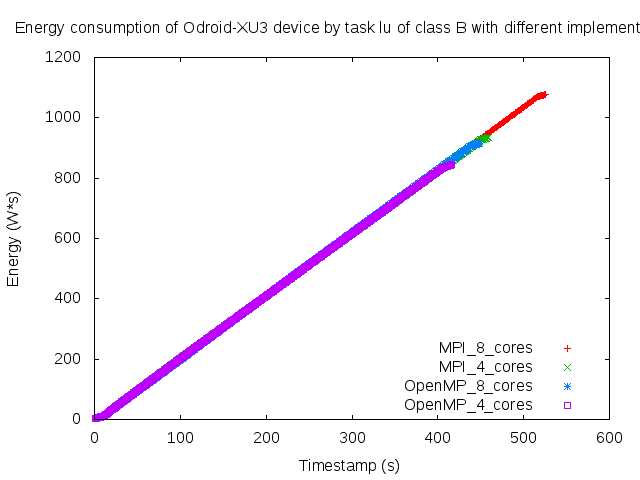
\includegraphics[width=\textwidth]{implementations_energy}
\caption[Energiebedarf und Implementationsmethode]{Energiebedarf und Implementationsmethode}
\label{fig:Energiebedarf und Implementationsmethode}
\end{figure}

Laut der Abbildungen \ref{fig:Leistung und Implementationsmethode} und \ref{fig: Energiebedarf und Implementationsmethode} kann man sagen, dass für diese Versuchtasks spielt OpenMP eine bessere Rolle als MPI, und zusätzlich ist der Durchlauf mit 4 Kerne besser als der mit 8 Kerne. Der Grund dafür kann nicht nur das sein, das im \ref{subsec:Energiebedarf und Architektur} geschieben werden hat, sondern auch wegen der Implementationsmethode. Weil ein lauffähige OpenMP-Programm während der Kompilierenphase in Parallelbereiche zugeordnet worden hat, jedes davon aus viele parallelausführbare Programmteil bestet. In der Durchlaufphase kann es sehr einfach in CPU-kerne zugeordernet. Aber die MPI-Programme brauch Kommunikation durch Peripherien, was eine höhere Zeit- und Energiebedarf verursacht.
